%% Settings for single-side (simplex) printing
% Margins: left 40mm, right 25mm, top and bottom 25mm
% (but beware, LaTeX adds 1in implicitly)
\documentclass[12pt,a4paper]{report}
\setlength\textwidth{160mm}

\usepackage[utf8]{inputenc}
\usepackage{graphicx}
\usepackage{fancyhdr}
\usepackage{lmodern}
\usepackage{lastpage}
\usepackage{subfig}
\usepackage{hyperref}

\graphicspath{{../graphs/}}

\pagestyle{fancy}
\fancyhf{}
\rhead{Petr Houška `houskape@gmail.com`}
\lhead{HW4: Hashing}
\rfoot{Page \thepage / \pageref{LastPage}}


\begin{document}
	
	\section{Náhodný testovací případ}
	\subsection{Počet kroků}
	\begin{figure}[h]	
		\centering	
		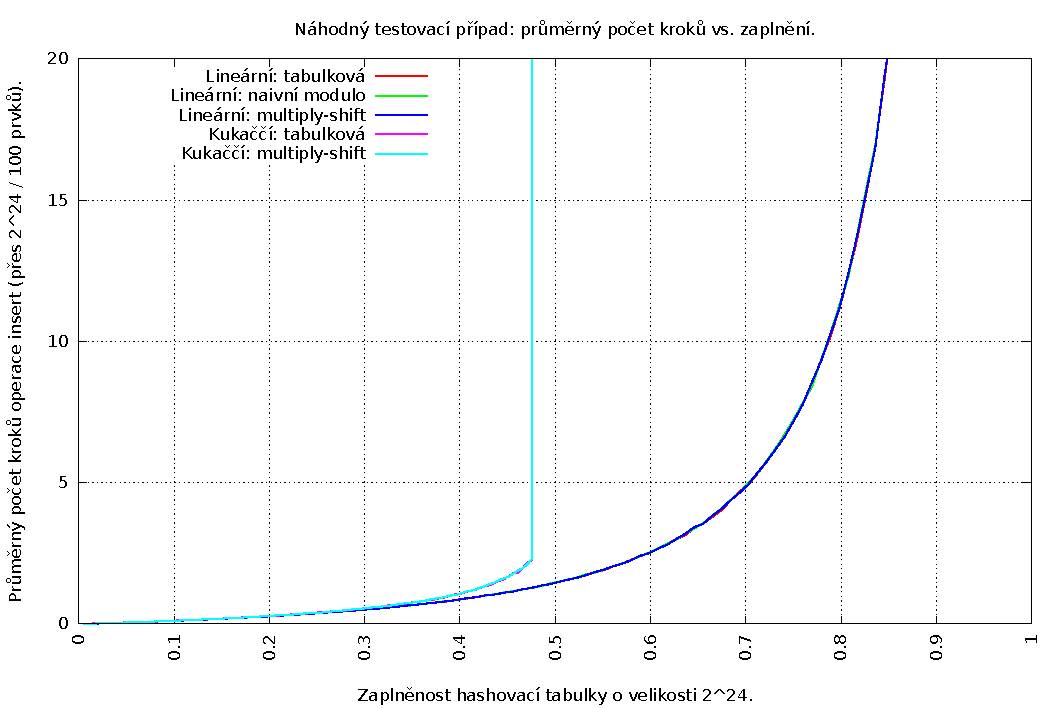
\includegraphics[scale=0.6]{graph_rand_steps}		
	\end{figure}

Na grafu průměrného počtu kroků jednotlivých hashovacích / kontejnorých algoritmů vidíme zejména dvě věci. Předně, pro náhodný vstup prakticky nezáleží na hashovací funkci, pouze na způsobu jak data do hashovacího kontaineru ukládámme. Jak u kukačky tak i u lineárního přidávání není v grafech pozorovatelný vůbec žádný rozdíl mezi hashovacími funkcemi. 

Tento výsledek si vysvětluji tím, že jsou-li už vstupní data "dokonale" náhodná, tak i vcelku špatná hashovací funkce (například naivní modulo v lineráním přidávání) nemůže, za předpokladu že je alespoň 1 nezávislá (tj. "nepreferuje nějakou přihrádku"), nic zkazit.

Druhý zajímavý jev je, že kukaččí hashování je - co se týče insertu - na počet operací striktně horší než linerání přidávání. Přibližně od zaplnění $48 \%$ pak složitost insertu vystřelí do  extrémních hodnot a pro zaplnení $50+ \%$ většinou ani nedoběhne. 

Namísto toho průměrný počet kroků na insert pro lineární přidávání roste sice exponsenciálně (alespoň to tak vypadá), ale ještě okolo zaplnění z $85 \%$ se drží na vceklu rozumných hodnotách ($<20$ kroků). Pro vyšší zaplnění průměrný počet kroků vystřeluje poměrně rychle k počtu příhrádek.

Poznámku si zaslouží, že kukaččí hashování může být ve skutečnosti pro zaplnění $<45 \%$ lepší i na počet kroků. Stačí při insertu vyzkoušet první hashovací funkci a pokud je jejím indexem určené políčko plné, tak neprovést hned swap, ale vyzkoušet ještě druhou funkci a swapovat až políčko určené tou. Tato drobná změna způsobí dvě věci. Předně posune průměrný počet kroků pro zaplnění $45 \%$ pod lineární přidávání a druhak trochu posune vystřelení nahoru (cirka o procento zaplnění).

	\subsection{Čas}

	\begin{figure}[h]	
	\centering	
	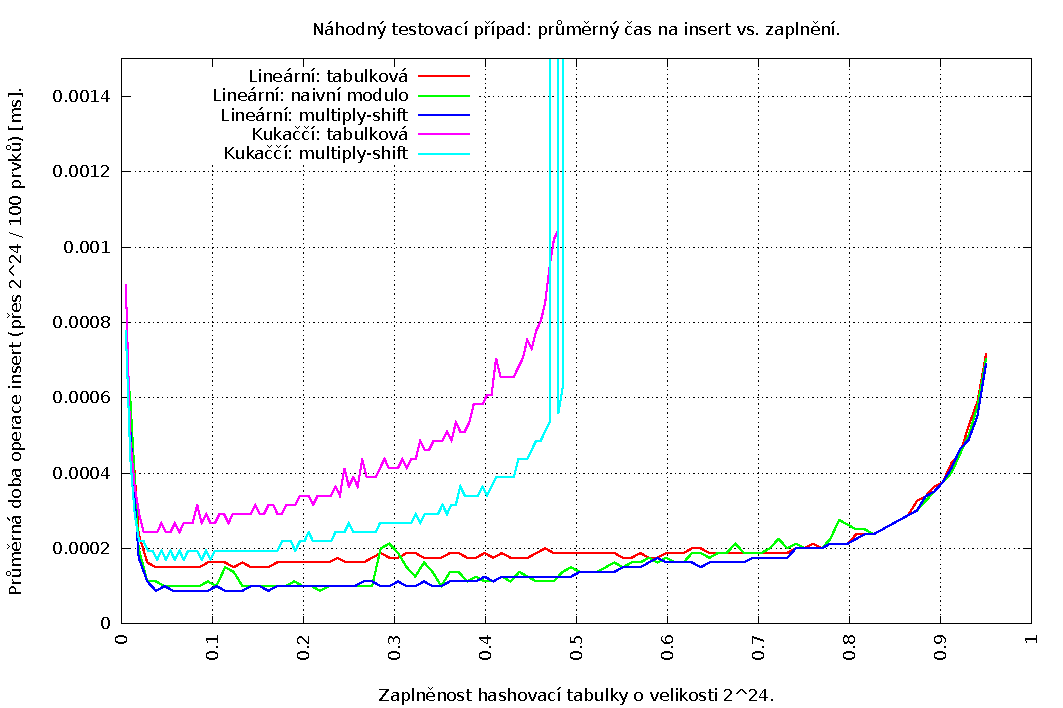
\includegraphics[scale=0.6]{graph_rand_time}		
	\end{figure}

V případě měření času na reálném hardwaru (i7-4712MQ CPU @ 2.30GHz, Turbo 3.0 GHz) jsou výsledky podobné průměrnému počtu kroků. Na rozdíl od počtu kroků se zde ale projevují rozdíly i mezi jednotlivými hashovacími funkcemi. 

Nepřekvapivě vítězí hashovací funkce, které je zjevně jednodušší spočítat. Pro lineární přidávání je konkrétně nejlepší naivní modulo, jen o málo horší (a ne vždy) je multiply-shift. A už s viditelným odstupem (byť pořád v řádově nižších desítkách procent) je tabulková hashovací funkce (konkrétně s tabulkami o 16bitových klíčích).

Stejný trend je i u kukaččího hashování, kde je tabulkové hashování taky pomalejší než multiply-shift. Nepřekvapivě je zde také rozdíl větší, a s zaplněním tabulky tolik neustupuje, jako je tomu u lineárního přidávání. Na rozdíl od lineárního přidávání je totiž s každým dalším krokem třeba hashovací funkci přepočítat. U lineráního přidávání se funkce počítá pouze jednou, další kroky jsou pouhé lookupy v poli bez nutnosti cokoliv počítat. 

To také vysvětluje důvod, proč u lineráního přidávání průměrný čas na insert roste výrazně pomaleji než průměrný počet kroků. Zatímco první spočítání funkce je vcelku náročná operace, tak testování lineárně za sebou jdoucích prvků pole na prázdnost je na moderním hardwaru s cachemi velmi rychlé. I extrémní počet kroků tak není pro lineární hashování takový problém, jak by se mohlo zdát.

Naproti tomu v případě kukaččího hashování znamená každý další krok spočítání hashovací funkce. Průměrný čas tedy roste s velmi podobným trendem jako průměrný počet kroků.

Výše zmíněné důvody jsou také, dle mého názoru, příčinou pro to, že je lineární přidávání rychlejší i na relativně malém zaplnění. Jediný krok v kukaččím hashování navíc (jediný swap) časově vydá za několik (desítek) kroků lineárního přidávání.

	\subsection{Další}
Třebaže by předchozí sekce mohly ukazovat, že kukaččí hashování nemá smysl, tak je nutné připomenout, že zde měříme nároročnost operace insert, zatímco hlavní výhoda kukaččího hashování tkví v konstantní náročnosti operace get. 
	
	\section{Sekvenční test}
	
		\begin{figure}[h]	
		\centering	
		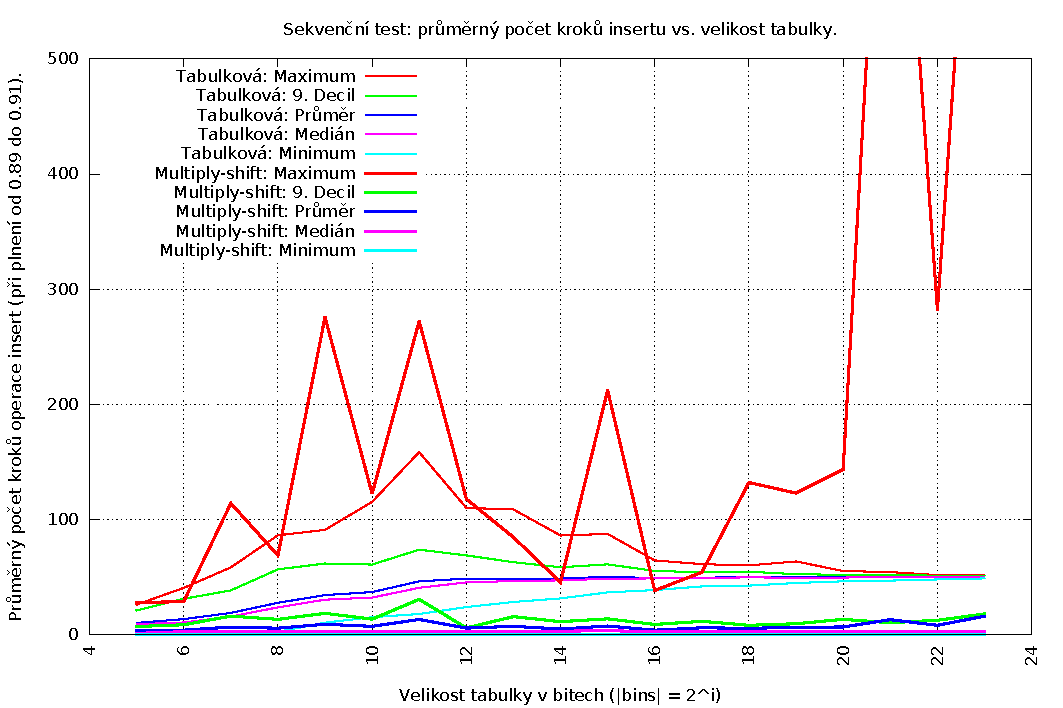
\includegraphics[scale=0.6]{graph_seq_both}		
	\end{figure}
	
	\begin{figure}[h]	
		\centering
		\subfloat{{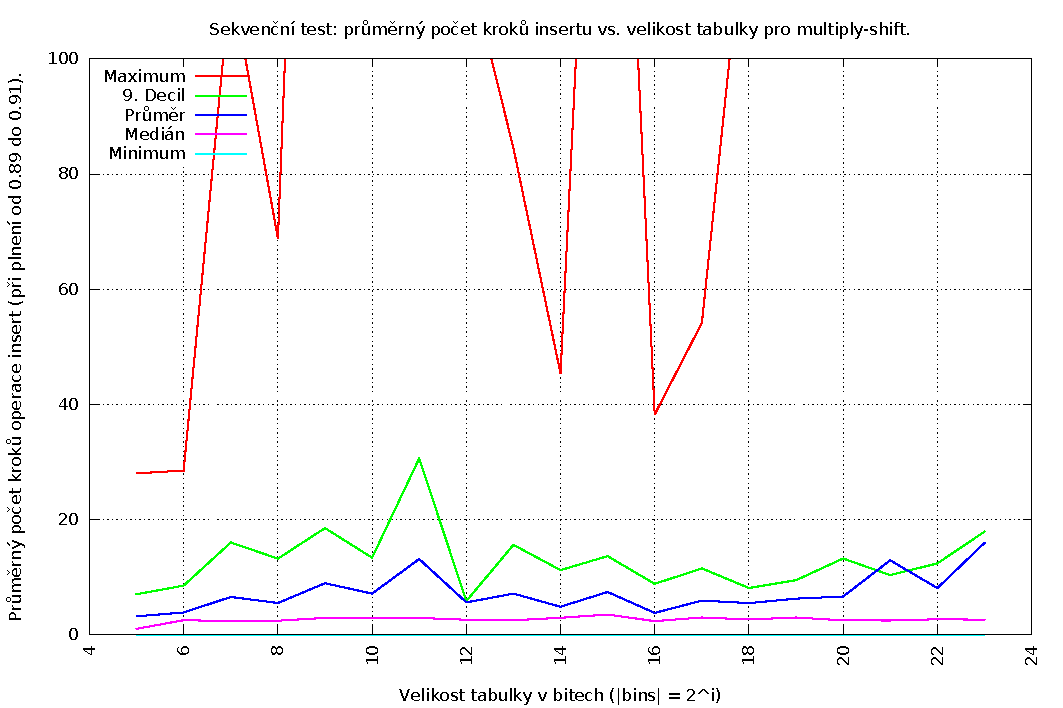
\includegraphics[scale=0.4]{graph_seq_multishift}	 }}%
		\qquad
		\subfloat{{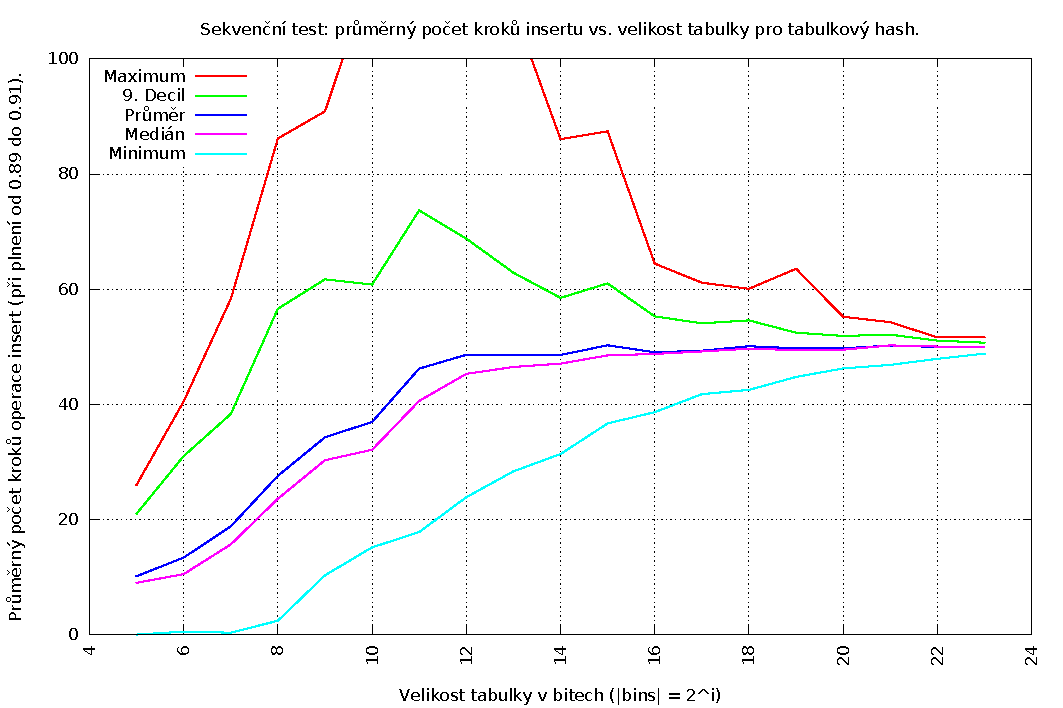
\includegraphics[scale=0.4]{graph_seq_table}	}}%
	\end{figure}
	
	Na rozdíl od náhodného testu v sekvenčním testu jsou vcelku jasně pozorovatelné rozdíly mezi hashovacími funkcemi, konkrétně mezi multiply-shift a tabulkovým hashováním.
	
	Tabulkové hashování je v téměř vždy horší než multiply-shift. Má horší (cirka $4x$) minimum, průměr, medián, i 9. decil. V případě maxima je ovšem situace jiná, tu má multiply-shift výrazně horší než tabulkové hashování. Jiný je také průběh průměrného počtu kroků vůči velikosti hashovacího kontaineru. 
	
	Zatímco v případě tabulkového hashování jednotlivé statistické ukazatele konvergují k jedné hodnotě (snižuje se rozptyl), tak u multiply-shift žádná taková tendence pozorovatelná není, spíše naopak.
	
	Obě pozorování si vysvětluji tím, jaká máme data v kombinaci s tím jak jednotlivé hashovací funkce fungují. 
	
	V případě multiply-shift na velikosti univerza do kterého hashujeme ani počtu hashovaných prvků prakticky nezáleží. Pro dostatečně velký (řádově > velikost hashovací tabulky) multiplikativní parametr $a$ bude rozhození vždy "dostatečně náhodné" a kolizí bude relativně málo. Ono pro "dostatečně velký multiplikativní parametr" je ovšem důležité. Pro malý paramtr "a" totiž naopak tento test dopadne extrémně špatně. 
	
	Vzhledem k sekvenčnosti vkládaných čísel je většina jejich horních bitů pro všechna stejná, pokud je tedy vynásobíme malým stejným číslem a použijeme - zas - jen horní bity, tak dostaneme stejná čísla. Pro špatně zvolené $a$ může být tedy multiply-shift velmi špatný, jak také ukazují data. 
	
	V případě tabulky se projevují stejné příčiny, ovšem jinak. Vzhledem k tomu, že všechna vkládaná čísla mají stejné horní bity, tak se při tabulkovém hashování projeví jen poslední tabulka / pár podleních tabulek. Pokud navíc hashujeme do malého počtu přihrádek, tak je velká šance, že ona poslední tabulka bude mít pro určité indexy stejné hodnoty. Tedy prakticky nedostaneme šanci využít celý prostor. S rostoucí velikostí hashovací tabulky ovšem vliv tohoto jevu slábne.
	
	Obecně horší je tabulkové hashování oproti multiply-shift kvůli tomu, že je-li (kvůli sekvenčnosti) použita vždy pouze poslední tabulka / poslední dvě, tak už z principu nedojde k využití celé hashovací tabulky. Multiply-shift tímto problémem netrpí. 
	
		



\end{document}